%% bpmlr.tex
%% V0.1
%% 2015/01/01
%% by Mack Sweeney

\documentclass[10pt]{proc}


% *** CITATION PACKAGES ***
%
\usepackage{cite}
% cite.sty was written by Donald Arseneau
% V1.6 and later of IEEEtran pre-defines the format of the cite.sty package
% \cite{} output to follow that of IEEE. Loading the cite package will
% result in citation numbers being automatically sorted and properly
% "compressed/ranged". e.g., [1], [9], [2], [7], [5], [6] without using
% cite.sty will become [1], [2], [5]--[7], [9] using cite.sty. cite.sty's
% \cite will automatically add leading space, if needed. Use cite.sty's
% noadjust option (cite.sty V3.8 and later) if you want to turn this off.
% cite.sty is already installed on most LaTeX systems. Be sure and use
% version 4.0 (2003-05-27) and later if using hyperref.sty. cite.sty does
% not currently provide for hyperlinked citations.
% The latest version can be obtained at:
% http://www.ctan.org/tex-archive/macros/latex/contrib/cite/
% The documentation is contained in the cite.sty file itself.


% *** OTHER BIBLIOGRAPHY PACKAGES ***
%
%\usepackage[numbers]{natbib}


% *** GRAPHICS RELATED PACKAGES ***
%
\usepackage[pdftex]{graphicx}
% declare the path(s) where your graphic files are
\graphicspath{{./graphics/}}
% and their extensions so you won't have to specify these with
% every instance of \includegraphics
\DeclareGraphicsExtensions{.pdf,.jpeg,.png}

\usepackage{scalerel}
\usepackage{mdframed}

% For graphical models:
\usepackage{tikz}
\usetikzlibrary{bayesnet}


% *** MATH PACKAGES ***
%
\usepackage[cmex10, fleqn]{amsmath}
\usepackage{bm}
\usepackage{amssymb}
% A popular package from the American Mathematical Society that provides
% many useful and powerful commands for dealing with mathematics. If using
% it, be sure to load this package with the cmex10 option to ensure that
% only type 1 fonts will utilized at all point sizes. Without this option,
% it is possible that some math symbols, particularly those within
% footnotes, will be rendered in bitmap form which will result in a
% document that can not be IEEE Xplore compliant!
%
% Also, note that the amsmath package sets \interdisplaylinepenalty to 10000
% thus preventing page breaks from occurring within multiline equations. Use:
\interdisplaylinepenalty=2500
% after loading amsmath to restore such page breaks as IEEEtran.cls normally
% does. amsmath.sty is already installed on most LaTeX systems. The latest
% version and documentation can be obtained at:
% http://www.ctan.org/tex-archive/macros/latex/required/amslatex/math/


% *** SPECIALIZED LIST PACKAGES ***
%
\usepackage{algorithm}
\usepackage[noend]{algpseudocode}


% *** ALIGNMENT PACKAGES ***
%
\usepackage{array}
\usepackage{booktabs}
% Frank Mittelbach's and David Carlisle's array.sty patches and improves
% the standard LaTeX2e array and tabular environments to provide better
% appearance and additional user controls. As the default LaTeX2e table
% generation code is lacking to the point of almost being broken with
% respect to the quality of the end results, all users are strongly
% advised to use an enhanced (at the very least that provided by array.sty)
% set of table tools. array.sty is already installed on most systems. The
% latest version and documentation can be obtained at:
% http://www.ctan.org/tex-archive/macros/latex/required/tools/


% *** SUBFIGURE PACKAGES ***
%\usepackage[tight,footnotesize]{subfigure}
% subfigure.sty was written by Steven Douglas Cochran. This package makes it
% easy to put subfigures in your figures. e.g., "Figure 1a and 1b". For IEEE
% work, it is a good idea to load it with the tight package option to reduce
% the amount of white space around the subfigures. subfigure.sty is already
% installed on most LaTeX systems. The latest version and documentation can
% be obtained at:
% http://www.ctan.org/tex-archive/obsolete/macros/latex/contrib/subfigure/
% subfigure.sty has been superceeded by subfig.sty.

%\usepackage[caption=false]{caption}
%\usepackage[font=footnotesize]{subfig}
% subfig.sty, also written by Steven Douglas Cochran, is the modern
% replacement for subfigure.sty. However, subfig.sty requires and
% automatically loads Axel Sommerfeldt's caption.sty which will override
% IEEEtran.cls handling of captions and this will result in nonIEEE style
% figure/table captions. To prevent this problem, be sure and preload
% caption.sty with its "caption=false" package option. This is will preserve
% IEEEtran.cls handing of captions. Version 1.3 (2005/06/28) and later 
% (recommended due to many improvements over 1.2) of subfig.sty supports
% the caption=false option directly:
\usepackage[caption=false,font=footnotesize]{subfig}



% *** FLOAT PACKAGES ***
%
\usepackage{fixltx2e}
% fixltx2e, the successor to the earlier fix2col.sty, was written by
% Frank Mittelbach and David Carlisle. This package corrects a few problems
% in the LaTeX2e kernel, the most notable of which is that in current
% LaTeX2e releases, the ordering of single and double column floats is not
% guaranteed to be preserved. Thus, an unpatched LaTeX2e can allow a
% single column figure to be placed prior to an earlier double column
% figure. The latest version and documentation can be found at:
% http://www.ctan.org/tex-archive/macros/latex/base/

\usepackage{stfloats}
% stfloats.sty was written by Sigitas Tolusis. This package gives LaTeX2e
% the ability to do double column floats at the bottom of the page as well
% as the top. (e.g., "\begin{figure*}[!b]" is not normally possible in
% LaTeX2e). It also provides a command:
%\fnbelowfloat
% to enable the placement of footnotes below bottom floats (the standard
% LaTeX2e kernel puts them above bottom floats). This is an invasive package
% which rewrites many portions of the LaTeX2e float routines. It may not work
% with other packages that modify the LaTeX2e float routines. The latest
% version and documentation can be obtained at:
% http://www.ctan.org/tex-archive/macros/latex/contrib/sttools/
% Documentation is contained in the stfloats.sty comments as well as in the
% presfull.pdf file. Do not use the stfloats baselinefloat ability as IEEE
% does not allow \baselineskip to stretch. Authors submitting work to the
% IEEE should note that IEEE rarely uses double column equations and
% that authors should try to avoid such use. Do not be tempted to use the
% cuted.sty or midfloat.sty packages (also by Sigitas Tolusis) as IEEE does
% not format its papers in such ways.


% *** PDF, URL AND HYPERLINK PACKAGES ***
%
\usepackage{url}
% url.sty was written by Donald Arseneau. It provides better support for
% handling and breaking URLs. url.sty is already installed on most LaTeX
% systems. The latest version can be obtained at:
% http://www.ctan.org/tex-archive/macros/latex/contrib/misc/
% Read the url.sty source comments for usage information. Basically,
% \url{my_url_here}.


% BEGIN PAPER CONTENT
%
\title{Probabilistic Personalized Multi-Linear Regression}
\author{
    Mack Sweeney, Kathryn Laskey, Huzefa Rangwala\\
        George Mason University
}
\date{\today}


% New commands to be used in this report.
\newcommand{\norm}[1]{\left\lVert#1\right\rVert}
\newcommand*{\Scale}[2][4]{\scalebox{#1}{$#2$}}%
\newcommand*{\Resize}[2]{\resizebox{#1}{!}{$#2$}}%
%\newcommand\scaleobj[2]{\hstretch{#1}{\vstretch{#1}{#2}}}


\begin{document}
\maketitle


\begin{abstract}

In \cite{elbadrawy_personalized_2015}, Elbadrawy et al. define a personalized
multi-linear regression model for predicting student performance in a
traditional university setting. This model is effectively a mixed-membership
linear regression with student-specific membership weights $P_s$ and bias terms
$b_s$ and course-specific bias terms $b_c$. In this paper, we will replicate
that model, derive an efficient SGD procedure for learning it, then define a
probabilistic formulation and derive an efficient Gibbs sampler for that
formulation.

\end{abstract}


\section{Introduction}

\paragraph{Outline}
The remainder of this paper is organized as follows.
Section~\ref{previous work} gives account of previous work.
Our new and exciting results are described in Section~\ref{results}.
Finally, Section~\ref{conclusions} gives the conclusions.


\section{Personalized Multi-Linear Regression (PMLR)}

Let $S$ be the set of all students in our database and $C$ be the set of all
courses in our database. Further, let $G$ be the matrix of all (student,ccourse)
dyads s.t. $G_{i,j}$ be the grade for student $i \in S$ in course $j \in C$.
Finally, let $I$ be an indicator matrix s.t. $I_{i,j} = 1$ if $G_{i,j}$ is a
dyad in our database (student $i$ has taken course $j$) and $I_{i,j} = 0$
otherwise. Our goal is to predict the grade a previously seen student will
achieve in a previously seen course. We do not attempt to make predictions for
cold-start records with this model. In order to facilitate conciseness of
notation, we define $n = |S|$ as the number of students, $m = |C|$ as the number
of courses, and $d = \sum_{i=1}^n \sum_{i=j}^m I_{i,j}$ as the number of
non-zero dyads $(i,j)$. Intuitively the model can be thought of as a linear
combination of one or more linear regression model outputs. So we additionally
define $f$ as the number of features and $M$ as the number of regression models.

The PMLR model is comprised of four parameters:

\begin{itemize}
    \item  $\bm{s}^{n x 1}$ is the vector of student bias terms
    \item  $\bm{c}^{m x 1}$ is the vector of course bias terms
    \item  $P^{n x M}$ is the matrix of student membership vectors
    \item  $W^{M x f}$ is the matrix of linear regression coefficient vectors
\end{itemize}

We make our observations for dyad features $\bm{X}_{i,j}^{f x 1}$ and make our
predictions with the function:

\begin{equation}
  \hat{g}(i,j) = \bm{s}_i + \bm{c}_j + P_i^T W \bm{X}_{i,j}.
\end{equation}

We say that the matrix $\hat{G}$ is the matrix of predicted grades, such that
$\hat{G}_{i,j} = \hat{g}(i, j)$.

The loss function is defined as the root mean squared error (RMSE):

\begin{equation}
  \mathcal{L}(i,j) = \norm{ G_{i,j} - \hat{G}_{i,j} }^2,
\end{equation}

and the squared Frobenius norm is used for regularization on the membership
weights $P_i$ and the regression coefficient matrix $W$:

\begin{equation}
  r(i,j) = \lambda (\norm{P_i}_F^2 + \norm{W}_F^2).
\end{equation}

Hence the overall objective function minimizes the sum of loss and the
regularization term:

\begin{equation}
    \underset{B, P, W}{\text{minimize}}
        \sum_{i=1}^n \sum_{j=1}^m
            I_{i,j} (\mathcal{L}(i,j) + r(i,j)).
\end{equation}


\subsection{Constraints}

In the original model, non-negativity constraints are placed on all model
parameters in order to enhance interpretability. These can be included if
interpretability is desired:

\begin{align}
  \begin{split}
    W_{l,k}  &\ge 0, 1 \le l \le M, 1 \le k \le f  \\
    P_{i,l}  &\ge 0, 1 \le l \le M, \forall i      \\
    \bm{s}_i &\ge 0, \forall i                    \\
    \bm{c}_j &\ge 0, \forall j
  \end{split}
\end{align}

\subsection{Stochastic Gradient Descent (SGD) Algorithm}

We now introduce an iterative SGD procedure for learning the parameters of the
model. We take partial derivatives of the objective function in terms of each
parameter. Let the error $E = \hat{G}_{i,j} - G_{i,j}$.

\begin{itemize}
  \item  $\bm{s}_i: 2E$
  \item  $\bm{c}_j: 2E$
  \item  $P_i: 2E(W \bm{X}_{i,j}) + 2\lambda P_i$
  \item  $W_l: 2E(P_i \bm{X}_{i,j}^T) + 2\lambda W$
\end{itemize}

So our algorithm is as follows:

\begin{algorithm}
  \caption{PMLR-SGD($\bm{X}, \alpha, \lambda, iters, M$) }
  \begin{algorithmic}[1]
    \State randomly init {$b^{(s)}, b^{(c)}, P, W$}
    \For{$iter$ in $iters$}
        \For{$\bm{X}_{i,j}$ in $X$}
            \State $\bm{s}_i = \bm{s}_i - \alpha * 2E$
            \State $\bm{c}_j = \bm{c}_j - \alpha * 2E$
            \State $P_i = P_i - \alpha * (2E(W X_{i,j}) + 2\lambda P_i)$
            \State $W = W - \alpha * (2E(P_i X_{i,j}^T) + 2\lambda W)$
        \EndFor
    \EndFor
  \end{algorithmic}
\end{algorithm}

The input parameters to this learning procedure include the learning rate
$\alpha$, the regularization multiplier $\lambda$, and the number of iterations
to learn for $iters$. We must also specify the number of models $M$.


\section{Bayesian Personalized Multi-Linear Regression (BPMLR)}

The PMLR model has several downsides. We observe that the learning
procedure requires four input parameters. The convergence of the algorithm is
highly dependent upon proper selection of the learning rate $\alpha$ and th
number of iterations $iters$. Too high a learning rate will cause divergence,
and too low a learning rate will slow learning considerably below the optimal
rate. The process of balancing divergence and speed of computation requires an
expensive grid search. While $iters$ can be removed with an early stopping
threshold, we are still replacing one parameter with another. Beyond convergence
issues, we must also perform an expensive grid search to find a proper setting
for $\lambda$ that adequately prevents model overfitting while still capturing
the valuable patterns in the data. Finally, the model selection process must
necessarily involve a grid search over values of $M$ as well as the other
parameters.

Our goal in a Bayesian formulation of this model is ultimately to remove
$\alpha, \lambda,$ and $M$. We will accomplish this in several steps. First we
will formulate a partially Bayesian PMLR model without substantial hierarhical
structure. This model will require several parameters to be set manually. Next
we will formulate a fully Bayesian version of the same model with hierarchical
hyperpriors. An efficient Gibbs sampler will be derived for this mddel. Instead
of the existing parameters, this sampler will take (1) number of burn-in
samples, (2) sample lag, (3) number of samples to generate, (4) a variety of
hyperparameters. Next we will explore the use of a Dirichlet Process (DP) to
automatically infer the optimal number of models $M$.

While we will actually end up with as many or more parameters as before, several
of these can be fixed across a variety of datasets and they will generally be
less difficult to set. The Bayesian model will achieve highly desirable
automatic complexity control and substantial interpretability increase over the
basic PMLR model.

\subsection{Probabilistic Formulation}

\mdfdefinestyle{eqbox}{
    innerleftmargin=5pt,
    innerrightmargin=5pt,
    innertopmargin=3pt,
    innerbottommargin=3pt
}


\begin{figure}[th!]
  \centering
  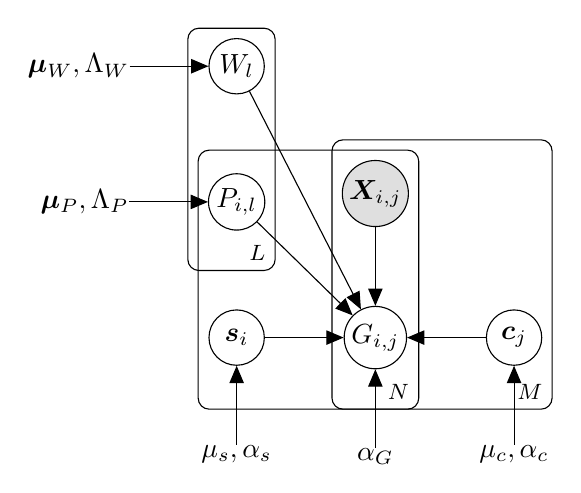
\begin{tikzpicture}

    % Define nodes
    \node[latent]                            (G) {$G_{i,j}$};
    \node[latent, left=of G]                 (s) {$\bm{s}_i$};
    \node[latent, right=of G]                (c) {$\bm{c}_j$};
    \node[latent, above=of s]                (P) {$P_{i,l}$};
    \node[latent, above=of P]                (W) {$W_l$};
    \node[obs, above=of G]                   (X) {$\bm{X}_{i,j}$};

    % G params
    \node[const, below=of G]  (pG) {$\alpha_G$};
    \edge {pG} {G};

    % s hyperparams
    \node[const, below=of s]  (Ts) {$\mu_s, \alpha_s$};
    \edge {Ts} {s};

    % c hyperparams
    \node[const, below=of c]  (Tc) {$\mu_c, \alpha_c$};
    \edge {Tc} {c};

    % P hyperparams
    \node[const, left=of P]   (TP) {$\bm{\mu}_P, \Lambda_P$};
    \edge {TP} {P};

    % W hyperparams
    \node[const, left=of W]   (TW) {$\bm{\mu}_W, \Lambda_W$};
    \edge {TW} {W};

    % Connect the nodes
    \edge {c,s,W,P,X} {G}; %

    % Plates
    \plate {student} {(s)(P)(G)(X)} {$N$};
    \plate {course} {(c)(G)(X)(student.north east)} {$M$};
    \plate {model} {(W)(P)(student.north west)} {$L$};

  \end{tikzpicture}
  \vspace{2pt}
  \caption{Bayesian PMLR Graphical Model} \label{fig:bpmlr-pgm}
\end{figure}


The likelihood of a particular grade $G_{i,j}$ is defined by:

\begin{equation}
    p(G | \bm{s}, \bm{c}, P, W, \alpha_G, \bm{X}) =
        \prod_{i=1}^n \prod_{j=1}^m
            \mathcal{N}(G_{i,j} | \hat{G}_{i,j}, \alpha_G),
\end{equation}

where

\begin{equation}
    \hat{G}_{i,j} = \bm{s}_i + \bm{c}_j + P_i^TW\bm{X}_{i,j}
\end{equation}

The four parameters $\bm{s}, \bm{c}, P, W$, and their hyperparameters are drawn
from the following distributions:

\begin{equation}
    p(\bm{s} | \mu_s, \alpha_s) =
        \prod_{i=1}^n \mathcal{N}(\bm{s}_i | \mu_s, \alpha_s)
\end{equation}

\begin{equation}
\begin{aligned}
    &p(\mu_s, \alpha_s | \mu_0, \kappa_0, \alpha_0, \beta_0) \\
        & = p(\mu_s | \alpha_s) p(\alpha_s) \\
        & = \mathcal{N}(\mu_s | \mu_0, (\kappa_0 \alpha_s))
            \Gamma(\alpha_s | \alpha_0, \beta_0)
\end{aligned}
\end{equation}

\begin{equation}
    p(\bm{c} | \mu_c, \alpha_c) =
        \prod_{j=1}^m \mathcal{N}(\bm{c}_j | \mu_c, \alpha_c)
\end{equation}

\begin{equation}
\begin{aligned}
    &p(\mu_c, \alpha_c | \mu_0, \kappa_0, \alpha_0, \beta_0) \\
        & = p(\mu_c | \alpha_c) p (\alpha_c) \\
        & = \mathcal{N}(\mu_c | \mu_0, (\kappa_0 \alpha_c))
            \Gamma(\alpha_c | \alpha_0, \beta_0)
\end{aligned}
\end{equation}

\begin{equation}
    p(P | \bm{\mu_P}, \Lambda_P) =
        \prod_{i=1}^n \mathcal{N}(P_i | \bm{\mu_P}, \Lambda_P)
\end{equation}

\begin{equation}
\begin{aligned}
    &p(\bm{\mu_P}, \Lambda_P | \bm{\mu_0}, \kappa_0, W_0, d_0) \\
        & = p(\bm{\mu_P} | \Lambda_P) p(\Lambda_P) \\
        & = \mathcal{N}(\bm{\mu_P} | \bm{\mu_0}, [\kappa_0 \Lambda_P])
            \mathcal{W}(\Lambda_P | W_0, d_0)
\end{aligned}
\end{equation}

\begin{equation}
    p(W | \bm{\mu_W}, \Lambda_W) =
        \prod_{l=1}^M \mathcal{N}(W_l | \bm{\mu_W}, \Lambda_W)
\end{equation}

\begin{equation}
\begin{aligned}
    &p(\bm{\mu_W}, \Lambda_W | \bm{\mu_0}, \kappa_0, W_0, d_0) \\
        & = p(\bm{\mu_W} | \Lambda_W) p(\Lambda_W) \\
        & = \mathcal{N}(\bm{\mu_W} | \bm{\mu_0}, [\kappa_0 \Lambda_W])
            \mathcal{W}(\Lambda_W | W_0, d_0)
\end{aligned}
\end{equation}


\subsection{Inference: Gibbs Sampler}

%% CPD for student bias vector: s
\begin{mdframed}[style=eqbox]
\begin{equation} \label{eqn:cpd-s}
\begin{aligned}
    &p(\bm{s}_i | \bm{c}, P, W, \bm{X}, G, \alpha_G, \Theta_s)
        = \mathcal{N}(\bm{s}_i | \mu_{s_i}^*, \alpha_{s_i}^*) \\
        & \sim \mathcal{N}(\bm{s}_i | \mu_s, \alpha_s)
               \prod_{j=1}^m \mathcal{N}(G_{i,j} | \hat{G}_{i,j}, \alpha_G)
\end{aligned}
\end{equation}

where

\begin{align}
    \alpha_{s_i}^* &= \begin{aligned}[t]
        \alpha_s + \alpha_G \sum_{j=1}^m I_{i,j}
    \end{aligned}\\
%
    \mu_{s_i}^* &= \begin{aligned}[t]
        \hstretch{0.8}{\vstretch{0.9}{
            \frac{
                \alpha_s\mu_s -
                \alpha_G \sum_{j=1}^m
                    [\bm{c}_j + P_i^TW\bm{X}_{i,j} - G_{i,j} ]^{I_{i,j}}}
            {\alpha_{s_i}^*}}}
    \end{aligned}
\end{align}
\end{mdframed}
%% END: CPD for s


%% CPD for course bias vector: c
\begin{mdframed}[style=eqbox]
\begin{equation} \label{cpd-c}
\begin{aligned}
    &p(\bm{c}_j | \bm{s}, P, W, \bm{X}, G, \alpha_G, \Theta_c)
        = \mathcal{N}(\bm{c}_j | \mu_{c_j}^*, \alpha_{c_j}^*) \\
        & \sim \mathcal{N}(\bm{c}_j | \mu_c, \alpha_c)
               \prod_{i=1}^n \mathcal{N}(G_{i,j} | \hat{G}_{i,j}, \alpha_G)
\end{aligned}
\end{equation}

where

\begin{align}
    \alpha_{c_j}^* &= \begin{aligned}[t]
        \alpha_c + \alpha_G \sum_{i=1}^n I_{i,j}
    \end{aligned}\\
%
    \mu_{c_j}^* &= \begin{aligned}[t]
        \hstretch{0.8}{\vstretch{0.9}{
            \frac{
                \alpha_c\mu_c -
                \alpha_G \sum_{i=1}^n
                    [\bm{s}_i + P_i^TW\bm{X}_{i,j} - G_{i,j} ]^{I_{i,j}}}
            {\alpha_{c_j}^*}}}
    \end{aligned}
\end{align}
\end{mdframed}
%% END: CPD for c


%% CPD for student membership matrix: P
\begin{mdframed}[style=eqbox]
{\setlength{\mathindent}{0cm}
\begin{equation} \label{cpd-P}
\begin{aligned}
    &p(P_i | \bm{s}, \bm{c}, W, \bm{X}, G, \Theta_P) =
        \mathcal{N}(P_i | \bm{\mu}_{P_i}^*, \Lambda_{P_i}^*) \\
        & \sim p(P_i | \bm{\mu_P}, \Lambda_P)
            \prod_{j=1}^m \mathcal{N}(G_{i,j} | \hat{G}_{i,j}, \alpha_G)
\end{aligned}
\end{equation}

where

\begin{align}
    \Lambda_{P_i}^* &= \begin{aligned}[t]
        \Lambda_P +
        \alpha_G W \left(
            \sum_{j=1}^m [\bm{X}_{i,j} \bm{X}_{i,j}^T ]^{I_{i,j}}
        \right) W^T
    \end{aligned}\\
%
    \bm{\mu}_{P_i}^* &= \begin{aligned}[t]
        \vstretch{0.9}{\hstretch{0.8}{
            [\Lambda_{P_i}^*]^{-1} \left(
                \Lambda_P\bm{\mu_P} +
                \alpha_G W \sum_{j=1}^m
                    [\bm{X}_{i,j}(G_{i,j} - \bm{s}_i - \bm{c}_j)]^{I_{i,j}}
            \right)}}
        \end{aligned}
\end{align}}
\end{mdframed}
%% END: CPD for P


%% CPD for regression coefficient matrix: W
\begin{mdframed}[style=eqbox]
{\setlength{\mathindent}{0cm}
\begin{equation} \label{cpd-W}
\begin{aligned}
    &p(W_l | \bm{s}, \bm{c}, P, \bm{X}, G, \Theta_W) =
        \mathcal{N}(W_l | \bm{\mu}_{W_l}^*, \Lambda_{W_l}^*) \\
        & \sim \mathcal{N}(W_l | \bm{\mu_W}, \Lambda_W)
            \sum_{i=1}^n \sum_{j=1}^m
                \mathcal{N}(G_{i,j} | \hat{G}_{i,j}, \alpha_G)
\end{aligned}
\end{equation}

where

\begin{align}
    \Lambda_{W_l}^* &= \begin{aligned}[t]
    \Lambda_W + \alpha_G \sum_{i=1}^N
        [ P_{i,l}^2 \sum_{j=1}^m
            \bm{X}_{i,j} \bm{X}_{i,j}^T ]^{I_{i,j}}
    \end{aligned}\\
%
    \bm{\mu}_{W_l}^* &= \begin{aligned}[t]
        \vstretch{0.9}{\hstretch{0.8}{
            [\Lambda_{W_l}^*]^{-1} \left(
                \Lambda_W\bm{\mu_W} +
                \alpha_G \sum_{i=1}^n
                    [P_{i,l} \sum_{j=1}^m
                        \bm{X}_{i,j}(G_{i,j} - \bm{s}_i - \bm{c}_j)
                    ]^{I_{i,j}}
            \right)}}
    \end{aligned}\\
    \nonumber
\end{align}}
\end{mdframed}
%% END: CPD for W

\subsection{Dirichlet Process Membership Vectors}


\section{Previous work}\label{previous work}


\section{Results}\label{results}
In this section we describe the results.


\section{Conclusions}\label{conclusions}
We worked hard, and achieved very little.


% use section* for acknowledgement
\section*{Acknowledgment}
This research was funded by NSF IIS grant 1447489.


\bibliographystyle{siam}
\bibliography{refs}

\end{document}

